% Very simple template for lab reports. Most common packages are already included.
\documentclass[a4paper, 11pt]{article}
\usepackage[utf8]{inputenc} % Change according your file encoding
\usepackage{graphicx}
\usepackage{url}
\usepackage{listings}
\usepackage{xcolor}

\definecolor{mygray}{rgb}{0.5,0.5,0.5}

\lstset{
    basicstyle=\footnotesize,
    language=erlang,
    frame=single,
    numbers=left,
    numberstyle=\tiny\color{mygray},
    breaklines=true,
}

%opening
\title{Loggy: a logical time logger}
\author{Antonios Kouzoupis $<$antkou$@$kth.se$>$}
\date{\today{}}

\begin{document}

\maketitle

\section{Introduction}

In this seminar we have implemented \emph{Loggy}, a logging server which prints
messages received in a logical order. For keeping a logical order in messages we
use the \emph{Lamport} timestamp algorithm. Every action performed in workers is
tagged with a timestamp and logger is responsible of ordering them.

In distributed systems, time is quite relative but (un)fortunately of great
importance. It is almost impossible to synchronize perfectly two or more clocks.
In a distributed system, different components communicate with each other by
exchanging messages so it is vital to keep a logical track of
``happened-before'' statement. An action in one process did happen-before
another one in another process.

\section{Main problems and solutions}

To address this issue in this assignment we use the \emph{Lamport} timestamp
algorithm. The algorithm itself was quite straightforward to implement. For
every message each worker sends, it increments its timestamp by one. For every
message a worker receives it increments by one the maximum of his counter and the
timestamp it received with the particular message. Nevertheless there were some
``grey areas'' whether we should increment the counter when a worker sends a
message to the logger. For example, after the worker waited for a random time,
it selects one of its peers and sends a message to it with the incremented
timestamp. It was unclear though if we should increment again the counter for
the message the worker sends to logger. After the instruction of our teaching
assistants I did not increment the counter twice. It would not make any
difference for the order, but it would just skip some numbers.

The tricky part of the assignment was for the logger to keep the logical time of
the messages it receives. It was obvious that we should keep the messages to a
queue so I made one list for every worker. The structure looks like that:

\begin{verbatim}
[{worker0, [Item00, Item01, ...]}, {worker1, [Item10, Item11, ...]}, ...]
\end{verbatim}

Where each \emph{Item's} structure is:

\begin{verbatim}
{From, Time, Msg}
\end{verbatim}

Again, each \emph{Msg} structure is:

\begin{verbatim}
{received/sending, Msg}
\end{verbatim}

So eventually the fundamental data structure of my logger looks like this:

\footnotesize
\begin{verbatim}
[{worker0, [{From00, Time00, {received, Msg00}}, {From01, Time01, {sending, Msg01}}, ..]},
{worker1, [{From10, Time10, {sending, Msg10}}, {From11, Time11, {received, Msg11}}, ..]}, ..]
\end{verbatim}
\normalsize

It is clear now that it was a very bad idea for my fundamental data structure to be so
complex. It made all the operations much more difficult.

My initial thought was to store every message to its respective message queue
according to the sender. After that I printed every message in the structure
that had Lamport time less than the message it was just received and delete them
from the structure. That solution gave me a ``more ordered'' output but still
some delayed messages were printed after those with bigger timestamp.

The second approach was after it stored a received message to the respective list,
it traversed all the message queues and found the minimum \emph{Lamport} time
of all. Then I printed only those messages in the queue with timestamp less than
the minimum and delete them from the list. Again, the messages were not printed
in the right order.

My final implementation was to check whether all the workers had sent messages.
So, first I check if all workers have messages in their queues -- have sent
messages to logger -- and then I get the minimum timestamp of all messages in
the structure. I print every message in all queues that has \emph{Lamport} time
less than or equal to the minimum and of course I remove them from the lists.
All those who have greater timestamp, are hold back for later evaluation.

\section{Evaluation}

For the evaluation process I run several tests with and without logical ordering
in logger. I mainly used the given test case with some minor changes. The test
bed had four workers, each one peering with the other three and one logger.

The first tests where obviously in the wrong order since the sending message was
logged after the received message and messages with high \emph{Lamport}
timestamp were printed before those with lower one. What was interesting was
that with lower values of jitter, messages seemed to be logged almost in the
right order, in terms that receiving and sending of the same message was logged
together. Of course timestamps were not in the right order but it was better
than tests with large jitter.

Later I introduced logical order functionality in the logger and the result was
what I expected. Messages with lower \emph{Lamport} timestamp were printed
before those with greater and sending message was logged before the received.
A typical output of an ordered log is illustrated in Figure \ref{fig:ordered}

\begin{figure}[h!]
\footnotesize
\begin{verbatim}
Logger: From: worker0 Lamport Time: 15 Message: {sending,{hello,57}}
Logger: From: worker0 Lamport Time: 16 Message: {sending,{hello,17}}
Logger: From: worker1 Lamport Time: 16 Message: {sending,{hello,16}}
Logger: From: worker2 Lamport Time: 16 Message: {received,worker0,{hello,57}}
Logger: From: worker0 Lamport Time: 17 Message: {sending,{hello,1}}
Logger: From: worker0 Lamport Time: 18 Message: {received,worker3,{hello,85}}
Logger: From: worker1 Lamport Time: 18 Message: {received,worker0,{hello,1}}
Logger: From: worker2 Lamport Time: 18 Message: {received,worker3,{hello,85}}
Logger: From: worker1 Lamport Time: 20 Message: {received,worker3,{hello,15}}
Logger: From: worker2 Lamport Time: 20 Message: {received,worker0,{hello,17}}
Logger: From: worker2 Lamport Time: 22 Message: {received,worker1,{hello,16}}
\end{verbatim}

\caption{In order logging}
\label{fig:ordered}
\end{figure}

What is really interesting is the length of the message queue. In Figure
\ref{fig:metrics} we can see that the message queue for all the workers is quite
small in relation to the number of messages. Of course it increases but not
proportional to the number of messages the logger has received.

\begin{figure}[h!]
\begin{center}
    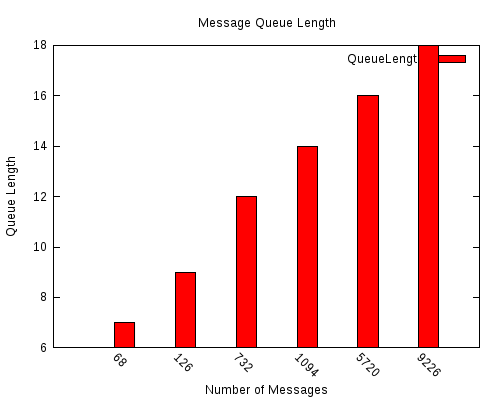
\includegraphics[scale=0.6]{queue_length.jpg}
    \caption{Length of Queue / Number of Messages}
    \label{fig:metrics}
\end{center}
\end{figure}

\section{Conclusions}

In this seminar we have implemented a logging service which receives messages
from multiple workers and has to print them in order. We used the \emph{Lamport}
algorithm to preserve the logical time and the ``happened--before'' relation. We
have also consolidated the great importance of time in distributed systems.
Finally, after these seminars I began feeling comfortable with Erlang.

\end{document}
